\documentclass[pdftex,12pt,letter]{article}
\usepackage[margin=0.75in]{geometry}
\usepackage{verbatim}
\usepackage{graphicx}
\usepackage[pdftex,pdfpagelabels,bookmarks,hyperindex,hyperfigures]{hyperref}

\newcommand{\fixme}[1]{\textbf{FIXME: #1}}    


\title{Design of the Data Management System for protoDUNE}
\date{\today}
\author{O. Gutsche, R. Illingworth, M. Mengel, A. Norman, M. Potekhin and B. Viren}

\begin{document}
\maketitle

\begin{abstract}
The protoDUNE detectors (dual-phase NA02 and single-phase NA04)
require a number of systems in order to marshal raw data from
their respective DAQ to prompt processing and mass storage.  This
document aims to  describe the general parameters of the problem, summarize the requirements
and explore a solution which involves leveraging F-FTS.
\end{abstract}

\tableofcontents

\pagebreak

\section{Overview}

\subsection{The protoDUNE program and detectors}
The protoDUNE program is designed for measurements with a test beam provided by a dedicated target and beamline system at the CERN SPS accelerator complex, and will help validate various DUNE technology aspects before proceeding with the construction of the principal DUNE detectors at SURF. It also has the potential to be an important platform for realistic LArTPC detector characterization (e.g. PID, shower response etc) utilizing controlled conditions of a test-beam experimental setup. The name ``protoDUNE'' currently applies to two full-scale LArTPC prototypes based on two different technologies. The ``full-scale'' designation is used to describe the fact that the prototypes contain important (and large) structural and readout elements built according to the specifications (including the size) of the eventual full detector.

The  ``single-phase'' (SP) LArTPC functions without amplification in the medium (liquid Argon) and is in essence a very large ionization chamber equipped with a large number of readout electrodes (wires), each with its own electronics chain. In this design, the front-end electronics is situated within the cryostat in order to minimize the noise (the so-called ``cold electronics design''). In the ``dual-phase'' (DP) TPC ionization electrons are extracted from liquid into gaseous phase of Argon, and drift in Argon gas towards a specially designed 2D structure on top of the detector where they multiply according to principles of proportional chamber operation. The two designs are complementary in the sense they explore different approaches to optimization of the Liquid Argon detector characteristics.

In December of 2015 the dual-phase prototype was given the official designation as a CERN experiment ``NP02'', and the single-phase was designated as ``NP04''. Both are to be deployed at CERN in 2017 and scheduled to take data in 2018. The prototypes will be placed in a specially constructed large-scale extension of the existing experimental hall located in the CERN North Area. Each prototype will be provided a dedicated optical fiber network connection to the CERN central storage facilities located in the West Area campus of CERN. The nominal bandwidth of these dedicated network connections will be 20 Gbps for each experiment. The motivations for this specific choice of nominal bandwidth will be presented in the following sections.

\subsection{Outlook for protoDUNE data characteristics}

In order to provide necessary precision for reconstruction of the ionization patterns in the LArTPC, both single-phase and dual-phase designs share the same fundamental characteristics:
\begin{itemize}
\item High spatial granularity of readout (e.g. the electrode pattern), and the resulting high channel count
\item High digitization frequency (which is essential to ensure precise position measurement along the drift direction)
\end{itemize}

\noindent
Another common factor in both designs is the relatively slow drift velocity of electrons in Liquid Argon, which is of the order of millimeters per microsecond, depending on the drift volume voltage and other parameters. This leads to substantial readout window (of the order of milliseconds) required to collect all of the ionization in the Liquid Argon volume due the event of interest. Even though the readout times are substantially different in the two designs, the net effect is similar in that due the the high digitization frequency in every channel (as explained above) this leads to a considerable amount of data per event.  Each event is comparable in size to a high-resolution digital photograph.

As will be shown in the following sections, it is foreseen that the total amount of data to be produced by the protoDUNE detectors will be of the order of a few petabytes (including commissioning runs with cosmic rays). Instantaneous and average data rates in the data transmission chain are expected to be substantial. For these reasons, capturing data streams generated by the protoDUNE DAQ systems, buffering of the data, performing fast QA type of analysis, transporting the data to sites external to CERN for processing (e.g. FNAL, BNL etc) requires resources and adequate planning.

\subsection{Prioritization}

All of the many elements in the chain of data acquisition, storage, distribution and processing are critically important in the sense that they are all required for the final results to be derived from the data. At the same time, protoDUNE has a critical dependency on the test beam availability (which is limited) provided by CERN and its schedule, which results in certains components of the data chain being more important than others in order to perform the measurements during a potentially limited time period. The priority components are the DAQ and the Raw Data Management System, which includes capturing the data coming out of the DAQ, transporting the data to persistent mass storage and prompt Quality Assurance which is required to ensure corrective action can be taken if the detector or certain system problems are identified in the QA process. The latter can be thought of as sophisticated monitoring done in near-time, which implies a ``few minute'' scale of processing.



\subsection{A note on the DAQ interface to the data handling system}

It is planned to have adequate buffering capability in the DAQ for both NP02 and NP04. In this case, “adequate” indicates in part conforming to a CERN requirement that the experiment must be able to keep taking data for a least 3 days at nominal rate, even if there is an occasional problem with the data link between the experiment site and CERN storage facilities, an issue with central storage or any type of similar outage. There is a difference in approach however in that
\begin{itemize}
\item Buffer depth in NP02 is larger, in order to make possible some processing right in the data room of the experiment. A number of middleware options are being explored for storage solution, in particular the BeeGFS file system.
\item In NP04 the emphasis is made on a more lightweight and fault tolerant which satisfies the general throughput requirement. No extensive processing is foreseen on the experiment site. Among the technical options for the buffer farm is xrootd.
\end{itemize}

\noindent
It is this “outer layer” of the data acquisition system in either experiment that will need to be interfaced with protoDUNE raw data management complex.




\section{Data Handling Parameters}
% appears to be orphaned

\subsection{Requirements}
The following is a summary of basic requirements for the protoDUNE data management system:
\begin{itemize}

\item Transfer raw data files from both online disk buffer farms of the DP and SP prototype detectors (NP02 and NP04 respectively) to CERN EOS disk and from there to CERN tape (CASTOR), FNAL tape (Enstore) and other end-points.

\item Ensure that the throughput is adequate and there are no bottlenecks for the Data Acquisition System given the expected data rates over the nominal two month running (see table)

\item Record metadata about file status and outcome of file operations

\item Operate at CERN and FNAL with support for initial setup and ongoing operations
\item Provide monitoring of overall system health, alerts on error and support debugging of problems.

\item Provide triggers to perform file operations (copy, delete) based on configurable rules

\item Support “express lane” process at CERN and other institutions.

\end{itemize}

\subsection{Data Characteristics}
The following table presents various characteristics of the data itself and of the data transmission system driven by the extreme
of each DP and SP detector and which the file handling system must accommodate on the assumption that they apply to both detectors.

\begin{table}[ht!]
	\centering
	\begin{tabular}{p{3.0in}p{0.95in}}
	\hline
	Total raw data & 2.5\,PB \\

	Total number of raw files & 2\,M \\

	Sustained data rate & 20\,Gbps \\

	Max latency to reach EOS & 10\,min \\

	Max latency to reach express processing & 10\,min\\

	Max simultaneous files in FTS dropbox & 1\,M\\

	Max simultaneous active files in transfer & 50,000\\

	Max file registrations & 200,000\,day$^{-1}$ \\


	\hline
\end{tabular}
\caption{protoDUNE data characteristics}
\label{tab:pdunedatachar}
\end{table}








\section{System Topology}
The baseline design for the online data handling system is shown schematically in Fig.\ref{fig:topology}.  This design leverages the technology of the Fermilab File Transfer Service (F-FTS) running in two positions within the CERN computing environment.


\begin{figure}[h]
  \centering
  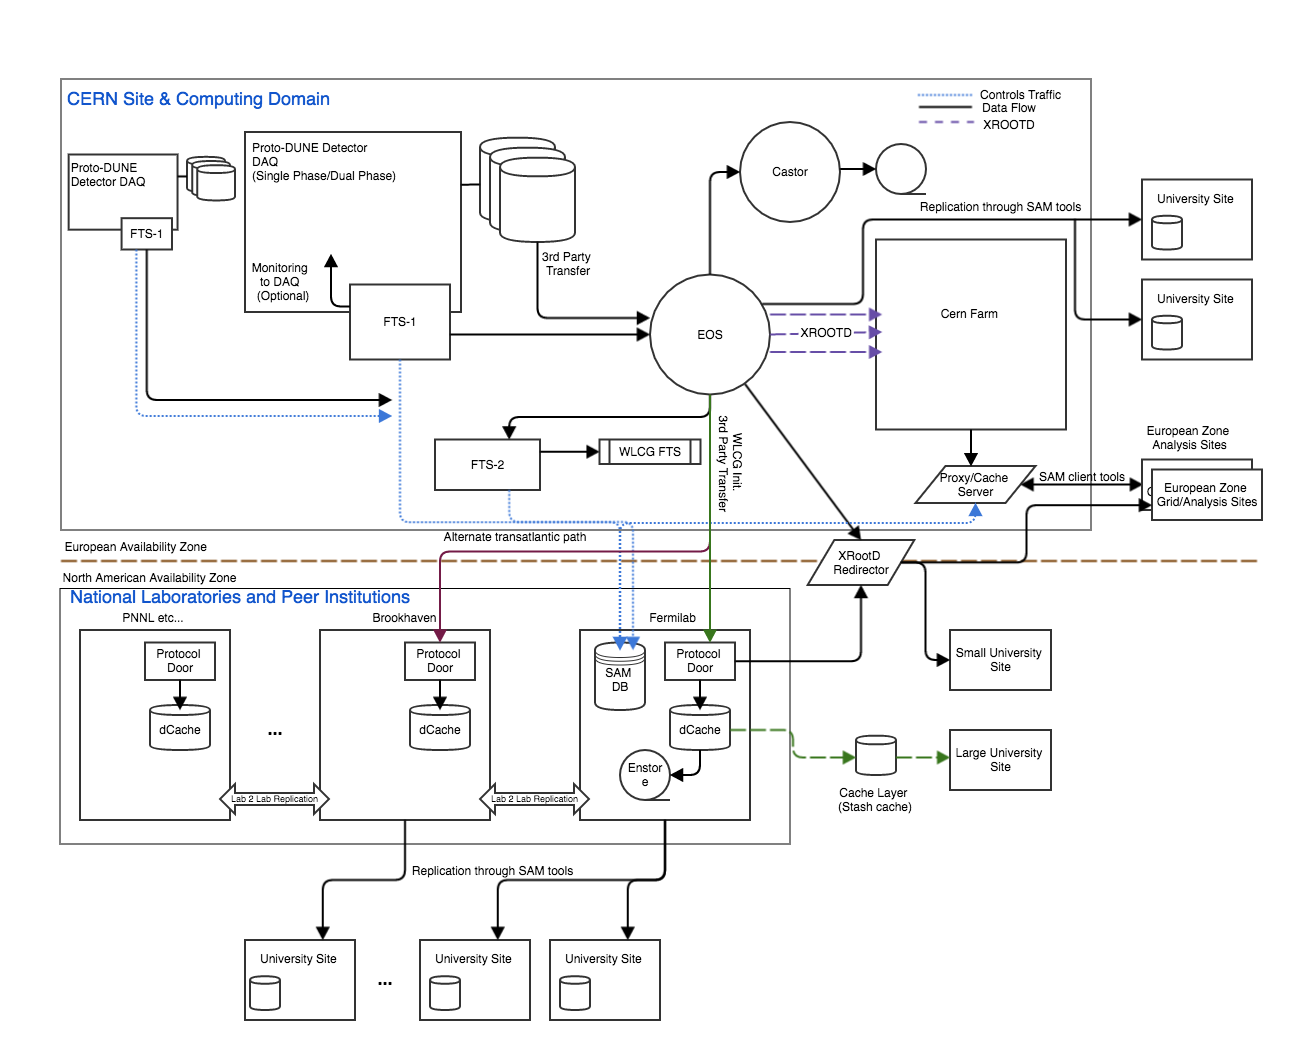
\includegraphics[width=1.0\textwidth]{protDune-datahandling-topology.png}
  \caption{Systems}
  \label{fig:topology}
\end{figure}

A primary F-FTS is homed within the protoDUNE DAQ domain for each of the detector setups (single phase or dual phase readout detectors) and is configured to run on a system which is able to access the DAQ’s buffer disks either through a POSIX filesystem or a protocol layer (e.g. XROOTD, gridFTP or others).  The primary FTS system is configured on this system to look at one or more input directories or storage locations, commonly referred to as a “dropboxes”.  The FTS daemon performs periodic scans of the configured dropboxes.  The system will operate asynchronously and independently of the protoDUNE DAQ systems.  When the protoDUNE DAQ has produced a file that it wishes to have passed off to the storage system, it will “move” (perform a filesystem/storage system atomic move operation or the equivalent) the file to the dropbox location. When a new file is located within one of the dropboxes, the system will initiate the file registration and transfer operations.


In the protoDUNE model, the primary FTS will initiate a copy operation from the online disk buffer farms into the EOS storage system.  The system will use the 3rd party copy support that is provided by the XROOTD protocol to allow for optimized transfers into EOS.  Upon completion of the initial copy into EOS, the FTS will initiate a “chained” copy (a copy that is dependent on the initial copy into EOS) of the data from EOS to the Castor archive system.  The FTS system will register each file’s metadata records (containing both basic and physics metadata, defined below)  in the SAM data handling system.  Upon completion of the replication of the data to Castor, the FTS will enter a monitoring/polling state of its operations to determine when the file has been successfully written to the archival media.
The primary FTS will handle the “cleanup” of its input dropbox.  The FTS performs configurable periodic cleanup passes through its current file sets.  The baseline cleanup logic is shown in Fig. X.  This cleanup process ensures that all files are successfully transferred and archived before they are deleted and provides an “age” criterion on files so that files can be retained within the DAQ environment for a period of time.  This allows operations like online/nearline processing or log files to be examined within the DAQ environment after the actual transfers to archival storage have completed.


The secondary FTS service runs outside of the detector DAQ domains, but within the CERN computing sphere.  This FTS system is configured to monitor as its input dropboxes, the EOS locations that the primary DAQ-FTS systems are using as output endpoints.  The system operates in the same manner as the primary FTS, scanning for new file and then initiating copy requests of the data to a set of one or more destination endpoints.  This FTS system will initiate the copy request between the European availability zone, and the North American availability zone.  At least one of the endpoint destinations for this service will be the FNAL-based dCache/Enstore system, where a second archival copy of the data will be recorded.  Additional copies across the availability zones can be configured based on available resources and available transatlantic bandwidth (e.g. direct transfer from CERN to BNL’s dCache or to PNNL’s storage facilities).  To perform the transfers, the F-FTS will interface with the WLCG FTS (as a supported transfer protocol) to schedule the actual transfer between the storage elements.  


\end{document}

%%% Local Variables:
%%% mode: latex
%%% TeX-master: t
%%% End:
